\documentclass[conference]{IEEEtran}
\usepackage{standalone}
\usepackage{times}
\usepackage{float}

%% Additional packages
\usepackage{times}
\usepackage{amsmath}
\usepackage{amsthm}
\usepackage{amssymb}
\usepackage{amsfonts}
\usepackage{mathtools}
%\usepackage{calc}
\usepackage{subfigure}
\usepackage{graphicx}
\usepackage{color}
\usepackage{url}
%\usepackage{lineno}
%\usepackage{ulem} % for underlining and strike through
%\normalem % reset emph to normal
%\usepackage{setspace} % for line spacing - e.g. 1.5, 2
\usepackage[usenames,x11names]{xcolor}
%\usepackage{xspace} % for inserting a space in TeX commands if needed
%\usepackage{caption}
\usepackage[bookmarks=true]{hyperref}
%\renewcommand{\thesubfigure}{\relax} % no subfig counters
%\let\chapter\section % algorithm2e natbib compatibility
%\usepackage{accents}
%\usepackage[titletoc,toc,title]{appendix}
%\usepackage{longtable}
%\usepackage{setspace}
\usepackage{multicol}

%% Packages
%\usepackage[margin=1in]{geometry}
%\usepackage[abs]{overpic}
\usepackage[linesnumbered,vlined,ruled]{algorithm2e}
%\usepackage{multirow} % for cell tables spanning multiple rows
\usepackage{tikz,pgf}%,tikz-3dplot}
\usetikzlibrary{arrows,automata,shapes,calc,backgrounds,spy,positioning}
%\usetikzlibrary{external}
%\tikzexternalize
%\usepackage[numbers]{natbib}
%\usepackage[sort,round]{natbib}
%\usepackage{lipsum}
\usepackage{epstopdf}

\theoremstyle{plain}
\newtheorem{theorem}{Theorem}
\newtheorem{cor}{Corollary}
\newtheorem{prop}{Proposition}
\newtheorem{lemma}{Lemma}

\theoremstyle{definition}
%\newtheorem{definition}{Definition}
\newtheorem{remark}{Remark}
\newtheorem{cond}{Condition}

\newtheorem{example}{Example}
\newtheorem{problem}{Problem}
%\newtheorem{assumption}{Assumption}


%%% figure path
\graphicspath{{figures/}}

%% Remove footnote mark
%\renewcommand{\footnotemark}{}

%%% Redefine qed symbol
%\renewcommand{\qedsymbol}{$\blacksquare$}

%% Projection symbol
%\newcommand{\project}[1]{\! \upharpoonright_{#1}}


%% Theorems 
%\newtheorem{theorem}{Theorem}[section]
%\newtheorem{proposition}[theorem]{Proposition}
%\newtheorem{corollary}[theorem]{Corollary}
\newtheorem{definition}[theorem]{Definition}
%\newtheorem{lemma}[theorem]{Lemma}
%\newtheorem{remark}[theorem]{Remark}
%\newtheorem{remarks}[theorem]{Remarks}
%\newtheorem{example}[theorem]{Example}
%\newtheorem{algo}[theorem]{Algorithm}
%\newtheorem{problem}[theorem]{Problem}
%\newtheorem{Procedure}[theorem]{Procedure}
%\newcommand{\exampler}[2]{\medskip \hskip -\parindent {\bf Example #1 Revisited.~}{\it #2}\medskip}

%% Percent
%\newcommand\oprocendsymbol{\hbox{$\square$}}
%\newcommand\oprocend{\relax\ifmmode\else\unskip\hfill\fi\oprocendsymbol}
%\def\eqoprocend{\tag*{$\bullet$}}

%% Enumerate environment
%\renewcommand{\labelenumi}{(\roman{enumi})}
%\renewcommand{\labelenumii}{(\alph{enumii})}

%% Breakable comma
%\mathchardef\breakingcomma\mathcode`\,
%{\catcode`,=\active
%  \gdef,{\breakingcomma\discretionary{}{}{}}
%}
%\newcommand{\breqn}[1]{\mathcode`\,=\string"8000 #1}

%% Other Stuff
%\newcommand{\margin}[1]{\marginpar{\tiny\color{blue} #1}}
%%\addtolength{\marginparwidth}{-0.3in}
\newcommand{\todo}[1]{\vskip 0.05in \colorbox{yellow}{$\Box$ \ttfamily\bfseries\small#1}\vskip 0.05in}
%\newcommand{\todo}[1]{}
%\newcommand{\vers}{\operatorname{vers}}

%% Roman, calligraphic, boldface, double barred letters
\newcommand{\RM}[1]{\mathrm{#1}}
\newcommand{\CA}[1]{\mathcal{#1}}
\newcommand{\BF}[1]{\mathbf{#1}}
\newcommand{\IT}[1]{\mathit{#1}}
\newcommand{\BB}[1]{\mathbb{#1}}
\newcommand{\TT}[1]{\mathtt{#1}}
\newcommand{\FK}[1]{\mathfrak{#1}}
\newcommand{\BS}[1]{\boldsymbol{#1}}

%%% Temporal logic symbols
\newcommand{\notltl}{\neg}
\newcommand{\andltl}{\wedge}
\newcommand{\orltl}{\vee}
\newcommand{\Next}{\ensuremath{\bigcirc}}
\newcommand{\Always}{\ensuremath{\ \square\ }}
\newcommand{\Event}{\ensuremath{\ \diamondsuit\ }}
\newcommand{\Until}{\ \CA{U}\ }
\newcommand{\Implies}{\Rightarrow}
\newcommand{\Equiv}{\Leftrightarrow}
%\newcommand{\Not}{\lnot}
\newcommand{\True}{\top}
\newcommand{\False}{\perp}
%\def\prop{\TT{data}}
%\def\popt{\pi}
\newcommand{\AP}{AP}
\newcommand{\pred}{\xi}

\newcommand{\Real}{\BB{R}}

%% Abbreviations
%\def\eg{e.g.\xspace}
%\def\Eg{E.g.\xspace}
%\def\ie{i.e.\xspace}
%\def\Ie{I.e.\xspace}
%\def\etc{etc.\xspace}
%\def\vs{vs.\xspace}
%\def\wrt{w.r.t.\xspace}
%\def\etal{et al.\xspace}

%% Exotic words
\newcommand{\buchi}{B\"uchi\ }

%% Symbols of automata
\newcommand{\PA}{\mathcal{P}}
\newcommand{\BA}{\mathcal{B}}
%\newcommand{\FA}{\mathcal{F}}

\newcommand{\TS}{\mathcal{F}}
\newcommand{\LA}{\mathcal{L}}
\newcommand{\KA}{\mathcal{K}}
\newcommand{\MDP}{\mathcal{M}}
\newcommand{\RA}{\mathcal{R}}
\newcommand{\FSA}{\mathcal{A}}

\newcommand{\TSX}{\BB{V}_\TS}
\newcommand{\TSE}{\BB{E}_\TS}
\newcommand{\TSEE}{\BB{E}}

\newcommand{\DTL}{DTL\xspace}


%% Short macros for arrows
\newcommand{\la}{\leftarrow}
\newcommand{\ra}{\rightarrow}
\newcommand{\ras}[1]{\stackrel{#1}{\rightarrow}}
\newcommand{\asgn}{\la}
\newcommand{\proj}[2]{{#1}{\downharpoonright_{#2}}}

\newcommand{\df}{\xspace\RM{d}}

%% Names of the Algorithms
%\newcommand{\optrun}{\textsc{Optimal-Run}\ }
%\newcommand{\exactmultioptrun}{\textsc{Exact-Multi-Robot-Optimal-Run}\ }
%\newcommand{\constR}{\textsc{Construct-Region-Automaton}\ }
%\newcommand{\constT}{\textsc{Construct-Team-TS}\ }
%\newcommand{\syncT}{\textsc{Sync-Team-TS}\ }
%\newcommand{\boundOpt}{\textsc{Bound-Optimality}\ }

% Custom operators
%\DeclareMathOperator*{\argmin}{arg\,min}
\newcommand{\norm}[1]{\left\| {#1} \right\|}
\newcommand{\norminf}[1]{\left\| {#1} \right\|_{\infty}}
\newcommand{\normeucl}[1]{\left\| {#1} \right\|_{2}}
\newcommand{\abs}[1]{\left| {#1} \right|}
\newcommand{\card}[1]{\left| {#1} \right|}
\newcommand{\spow}[1]{2^{#1}}
%\newcommand{\interior}[1]{\accentset{\smash{\raisebox{-0.12ex}{$\scriptstyle\circ$}}}{#1}\rule{0pt}{2.3ex}}
\newcommand{\interior}[1]{\mathring{#1}}
\DeclareMathOperator{\diag}{diag}
\newcommand{\lift}{\upharpoonright}
%
%% Display a grid to help align images
%\beamertemplategridbackground[1cm]
%\usepackage[style=numeric-comp]{biblatex}
\usepackage{cite}


%\documentclass[letterpaper, 11pt, onecolumn]{TemplateFiles/ieeeconf}
%\IEEEoverridecommandlockouts \overrideIEEEmargins 
%\pagestyle{plain}

%\usepackage[ruled,vlined,linesnumbered,boxruled]{algorithm2e}
%\usepackage{mathrsfs}
%\usepackage{graphicx}
%\usepackage{amsfonts}
%\usepackage{amsmath}
%\usepackage{amssymb}
%\usepackage{array}
%\usepackage{flafter}
%\usepackage{tabu}
%\usepackage{cite}
%\usepackage{subfigure}
%\usepackage{verbatim}
%\usepackage{bbm}
%\usepackage[usenames]{color}
%\usepackage[svgnames]{xcolor}

%\usepackage{balance}

%\usepackage{nicefrac}
%\usepackage{psfrag}
%\usepackage{umoline}
%\usepackage{hyperref}
%\usepackage{appendix} %[2009/09/02 v1.2b extra appendix facilities]
%\let\proof\relax
%\let\endproof\relax
%\usepackage{amsthm}	% This is needed for \newtheorem and proof environment.
% \usepackage{natbib} % for citing the papers with auther-year format in parantheses.
%\usepackage[numbers, sort]{natbib}

%\usepackage{etoolbox}

%\providecommand{\citet}[1]{\citeauthor{#1}\,[\citeyear{#1}]}
%\providecommand{\citep}[1]{\cite{#1}}

%\newtheorem{thm}{Theorem}
%\newtheorem{Def}{Definition}
%\newtheorem{Problem}{Problem}
%\newtheorem{Lem}{Lemma}
%\newtheorem{Cor}{Corollary}
%\newtheorem{assumption}{Assumption}
%\newtheorem{proposition}{Proposition}
%\newtheorem{definition}{Definition}
%\newtheorem{property}{Property}
%\newtheorem{Remark}{Remark}
%\newtheorem{exmp}{Example}[section]
%\newenvironment{proof}[1][Proof]{\begin{trivlist}
%\item[\hskip \labelsep {\bfseries #1}]}{\end{trivlist}}

%\newcommand{\TypeOfDoc}{IJRR} % This either can be TR or Conf or IJRR
%\newcommand{\FinalFlag}{No} % This either can be No or Accepted
%\newtoggle{finalpaper}
%\toggletrue{finalpaper}
%\togglefalse{finalpaper}

\graphicspath{{./figs/}}

%\allowdisplaybreaks[1]

%\newcommand{\kXX}[1]{\color{blue} XX #1 XX \color{black}}
%newcommand{\AXX}[1]{\color{purple} XX #1 XX \color{black}}
\newcommand{\aXX}[1]{\color{orange} #1  \color{black}}
\newcommand{\axx}[1]{\aXX{#1}}


\newcommand{\pr}[1]{\textbf{#1:} }

\newcommand{\codeline}[1]{\par{\ttfamily #1 \par}}  % This line is added because sth like this \newcommand{\initeali}{\verb|InitializeEdge|} does not work. For further details please check out this link % http://tex.stackexchange.com/questions/86071/newcommand-for-verbatim
% please do not delete above comments as it can be really confsing


%%%%%%%%%%%%%%%% symbols
\newcommand{\tv}{\varpi} % tube volume (edge tube volume)
\newcommand{\td}{\Gamma} % tube distance (edge tube distance)

%%%%%%%%%%%%%%%%%%%%%%%%%%%%%%%%%%%%%%%%%%%%%%%%%% To reduce pages
%\textfloatsep = 0pt
%\renewcommand{\baselinestretch}{0.96}
%%%%%%%%%%%%%%%%% Make bibs smaller
%\renewcommand{\IEEEbibitemsep}{0pt plus 2pt}
%\makeatletter
%\IEEEtriggercmd{\reset@font\normalfont\footnotesize}
%\makeatother
%\IEEEtriggeratref{1}

%%%%%%%%%%%%%%%%% margins
%\usepackage{geometry}
% \newcommand{\papermargin}{0.97in} % IEEE asks for 0.75 on all pages, but the first page
% %\newgeometry{top=0.75in,bottom=.75in,right=.75in,left=.75in}
% \newgeometry{top=\papermargin,bottom=\papermargin,right=\papermargin,left=\papermargin}
% \newgeometry{top=1.in,bottom=1.in,right=1.in,left=1.in}

\let\labelindent\relax
\usepackage{enumitem}


% numbers option provides compact numerical references in the text. 

\pdfinfo{
   /Author (Homer Simpson)
   /Title  (Robots: Our new overlords)
   /CreationDate (D:20101201120000)
   /Subject (Robots)
   /Keywords (Robots;Overlords)
}

% Table caption wrangling
\usepackage{etoolbox}
\makeatletter
\patchcmd{\@makecaption}
  {\scshape}
  {}
  {}
  {}
\makeatletter
\patchcmd{\@makecaption}
  {\\}
  {.\ }
  {}
  {}
\makeatother

\newcommand{\Ali}[1]{{\color{green} Ali: #1}}
\newcommand{\cristi}[1]{{\color{orange} Cristi: #1}}
%\newcommand{\rohan}[1]{{\color{blue} Rohan: #1}}
\allowdisplaybreaks[1]

\begin{document}

% paper title
%\title{\large From Mission Specification to Safe Control Logic Under Uncertainty:\\ Application to Mars Copter-Rover Navigation-Coordination}

\title{\huge Software/Systems}

\author{Kyon, Rohan, Petter, Kamak, Cristi, Sofie, Ali Agha, Richard Murray, Aaron Ames}

\maketitle

\begin{abstract}
This report summarizes the software architecture and the system description for V\&V tasks. 
\end{abstract}

\IEEEpeerreviewmaketitle

	
%%%%%%%%%%%%%%%%%%%%%%%%%%%%%%%%%%%%%%%%%%%%%%%%
%%%%%%%%%%%%%%%%%%%%%%%%%%%%%%%%%%%%%%%%%%%%%%%%
\section{Introduction} \label{subsec:intro}

To verify the validity of the algorithms, we have built an end-to-end system based on ROS (Robot Operating System). Each module in the system communicates each other using the predefined message types over ROS's synchronous/asynchronous communication infrastructure. The modular architecture provides an abstraction of hardware, which enables testing with both hardware and simulation using the same code base. 

\section{Software Architecture}

A high-level software architecture is shown in Fig.~\ref{fig:software_arch}. Each node in the graph roughly corresponding to a single ROS node (process). The background color represents the status of node development. 

\textit{Belief space planner} is a core planning node running on the ground vehicle. It takes a map from the copter (and possibly from rover's navigation cameras) as input, and generates a policy for the rover's motion and next measurement plans for the copter. 

\textit{Policy executor} receives the policy from the planner, and translates the policy to the form that the locomotion node can understand (e.g., next waypoint coordinates).

\textit{Locomotor} accepts two types of commands: arc and waypoint. The arc command directly specifies three arc parameters, namely length, angle change, and direction . The waypoint command specifies $x$ and $y$, with the option of additional heading $\theta$. 

\textit{Pose estimator} is an EKF fusing the information from motor commands, an IMU, and cameras. The estimator gives a mean pose estimate with covariance.


The other modules are mock at this moment. The descriptions will be updated as they proceed. 




\subsection{Simulation}

We use the Gazebo simulation framework\footnote{http://gazebosim.org}, which comes with physics and graphics computation engines with potential ROS integration. We chose Gazebo over the JPL in-house simulation framework (DARTS) for the ease of multi-institutional collaboration. 

Our focus in the simulation is sorely on the validation of the planning pipeline, rather than high-fidelity physics-based evaluation. Therefore, simplified models will be used wherever reasonable.

\subsection{Environmental Models}

\begin{figure}
    \centering
    %\includegraphics[width=\textwidth]{BeliefSpaceTemporalLogic/figs/GazeboScene}
    \caption{Mars terrain loaded in the Gazebo simulator}
    \label{fig:gazebo_scene}
\end{figure}

We use Martian terrain models from the JPL OnSight project. Their map processing pipeline produces photo-realistic terrain geometry from MSL Curiosity's surface imagery. An example scene is shown in Fig.~\ref{fig:gazebo_scene}.

\subsection{Robot Models}
TBD


\section{Hardware Testbed}

\subsection{Ground rover (Athena/JPL)}


\subsection{Aerial copter (Caltech)}



\section{Scenario}
\begin{itemize}
  \item Map Building
  \item Map Labelling
\end{itemize}

\begin{figure}[th!]
	\centering
	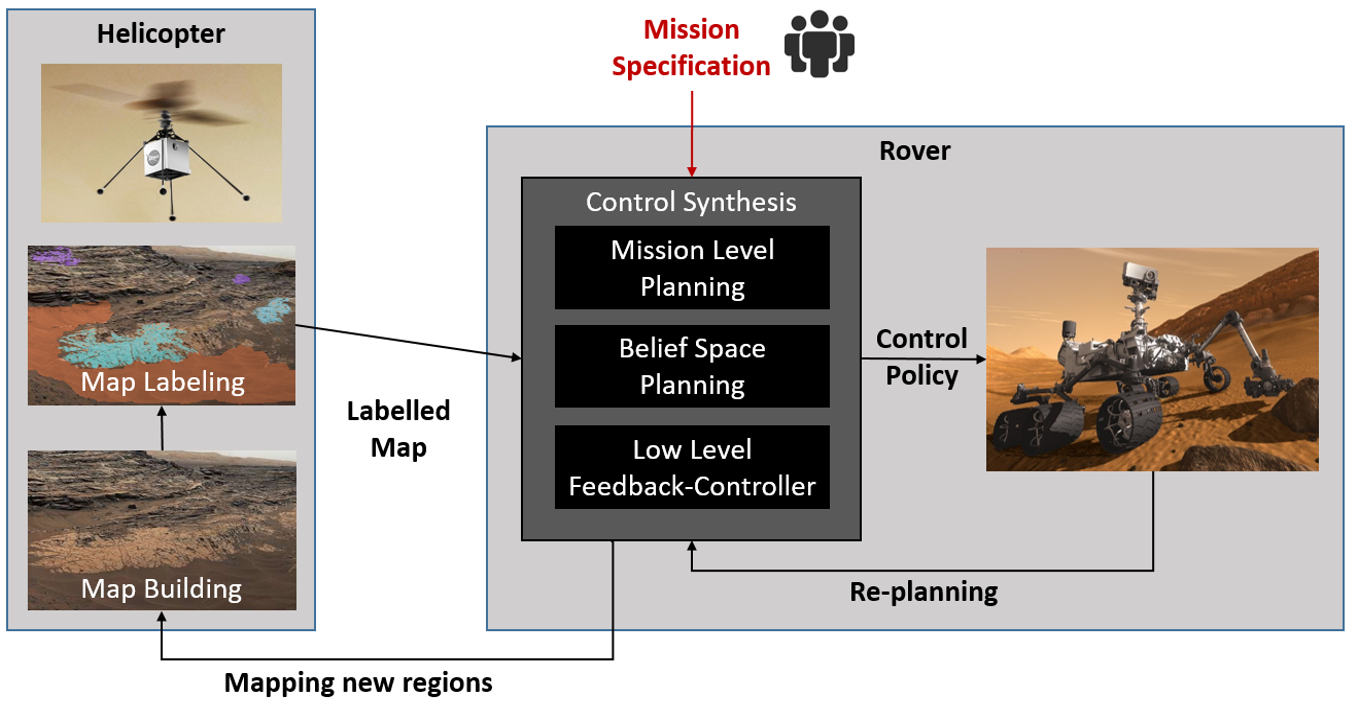
\includegraphics[width=\columnwidth]{figs/FunctionalArcV4.png}
	\caption{Architecture showing mapping, planning and execution framework.}
	\label{fig:FuncArc}
\end{figure}    	

%%%%%%%%%%%%%%%%%%%%%%%%%%%%%%%%%%%%%%%%%%%%%%%%%%%%%%%%%%%%%%%%%%%%%%%%%%%%%%%%%%%%%%%%%%%%%%%%%%%%%%%%%%%%%%
\begin{figure*}
    \centering
    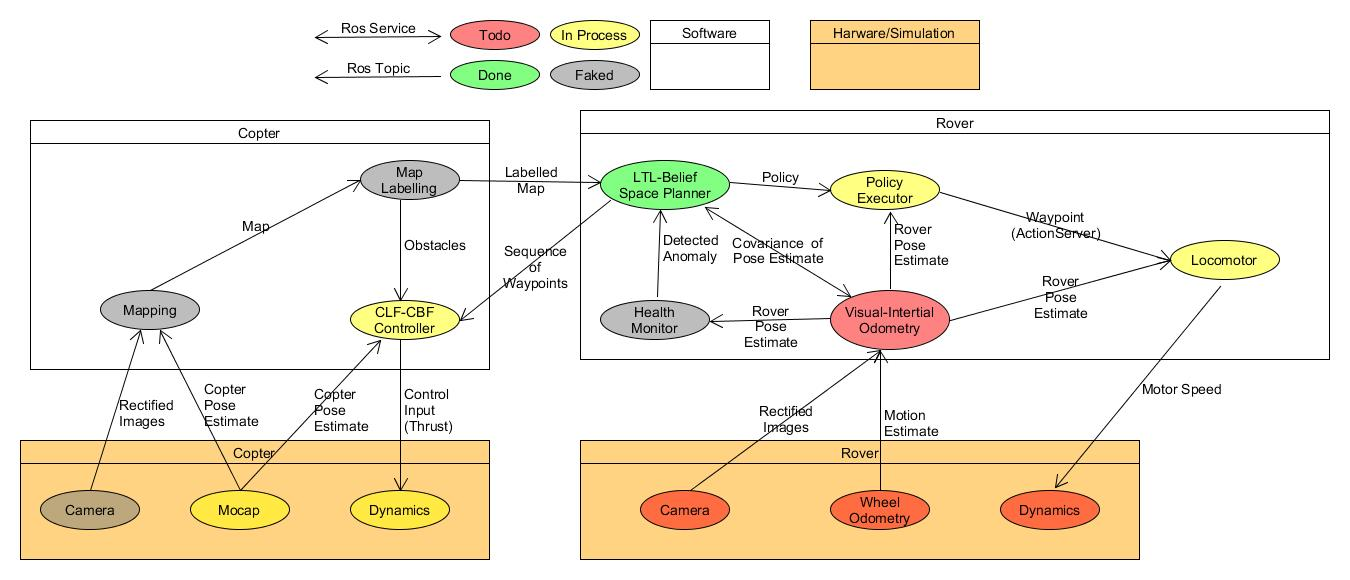
\includegraphics[width=\textwidth]{BeliefSpaceTemporalLogic/figs/SoftwareArch.jpg}
    \caption{Software architecture}
    \label{fig:software_arch}
\end{figure*}



\section{Development Status}

Below is the development status as of December 11.

\subsection{Core Navigation Modules}

\subsubsection{Perception}

\paragraph{Stereo Reconstruction (complete)}
The JPLV stereo vision has been implemented. It provides point cloud up to 7-8m. 

\paragraph{Terrain Classification (development complete; copter test requires 1 week; multi-class extention requires 1+ month)}
The SPOC-lite classifier provides the probability (confidence) of sand given a single color image. The SPOC-lite is essentially a 5-class classifier based on SVM Linear \cite{liblinear}. It is specialized to detect the white sand regions in the JPL Mars yard (the accuracy is $>$98\%).

As it is trained for rover's downward-looking mast camera, the performance is unknown for copter's imagery. The Mars yard test requires about a week. 

Extra labeling and training may be required for the following cases: reliable multi-class classification, classification in different environment (e.g., JPL mini Mars yard, Caltech wind tunnel). 


\paragraph{Traversability Assessent (complete; adaption requires up to 2-3 days)}
The Morphin traversability analyzer (the ancestor of MER/MSL GESTALT) is implemented. The adaptation to different terrain requires intensive parameter tuning. For stable performance, 2-3 day testing will be required.


\subsubsection{State Estimation}

\paragraph{Visual Odometry (complete)}
The JPL VO provides 6DoF pose information in 3.75 Hz. 

\paragraph{IMU (2 weeks)}
An IMU is mounted on Athena, but the sensor does not publish any data in the ROS space. There is a plan to install a new IMU but it is currently under testing on a benchtop model.

\paragraph{EKF (2-3 months?; 2-3 weeks for 3rdparty option)}
There is an effort to implement an EKF that fuses wheel odometry, visual odometry, and IMU. It is under testing on a benchtop model. No ROS wrapper presents.

On special need,  the 3rdparty EKF like robot\_localization\footnote{\url{http://wiki.ros.org/robot_localization}} may be installed. This will use VO and WO as odometry input. The integration and testing requires about 2-3 weeks.


\subsubsection{Actuation}

\paragraph{Locomotion (complete; 2 weeks to implement visual feedback; 3 months for proper velocity distribution over articulated suspention)}
The locomotion module drives a rover to a designated point. The destination is specified either by $ (x, y, \theta) $ or arc parameters. Each wheel is separately controlled in terms of position and velocity.

The vision-based path tracking is not implemented. It requires about two weeks to implement and test. 

The suspension model is not incorpolated into the velocity distribution to six wheels. Therefore, actuation error may be innegligible in undulating terrain. This requires suspention angle measurements which are not possible with the current hardware configurations. 


\paragraph{Mast Actuation (complete)}
The mast actuation module moves the mast gymbal to a designated direction. The direction is specified using the cartesian coordinates (XYZ) or joint angles (azimuth and elevation). 



\subsection{Gazebo Simulation}

\paragraph{Environmental Model (visual complete; physical 1 week)}
Realistic Martian terrain models are already available in Gazebo. If physical interaction is needed, surface parameters should be tuned to produce natural rover motions. 

\paragraph{Rover Model (1 week for visual; 2 weeks for physical)}
The rocker-bogie rover model is not available in DARTS. The visualization takes about a week to move the vehicle parts (suspention, wheels). 

The physical model is completely unavailable. Porting from DARTS models should take about 2 weeks.

\paragraph{Copter Model (quadcopter visual available; helicopter visual 1 week; 3 day to emulate heli camera; 1-2 months for full aerodynamics simulation)}
The estimate work time for the mock helicopter is one week. If it requires full simulation (I hope not), it will take months. 


\subsection{DARTS Simulation}

Generally, using DARTS requires a steep learning curve. For those who don't have experience with DARTS, it takes 1-2 more months in learning before working on practical tasks. 

\paragraph{Environmental Model (visual 1 week; physical 1 week)}
The same Martian model may be installed onto the DARTS environment as well. It takes up to two weeks to fully integrated in the system.

\paragraph{Rover Model (complete)}
Various rocker-bogie rover models are available as a part of ROAMS.

\paragraph{Copter Model (1-2 weeks?)}
A few copter models are available as a part of DSENDS. It may take 1-2 weeks to learn to control copters.

\paragraph{ROS interface (3 weeks)}
Significant effort needed to connect DARTS simulator with the ROS interface. There is a prototype implementation for ROAMS. It will take about 3 weeks to expose all relevant functionalities to ROS.


\subsection{Decision}
As of December 12, we decided to go with the simulation only (possibly with Gazebo). The estimate work time is about 10 weeks (around the end of February). 

This is not the final decision. As the project proceeds, we may make a replan based on the belief we have at the point. We will review the progress at roughly each end of months. 


\begin{thebibliography}{99}
\bibitem{liblinear}
LIBLINEAR, \url{https://www.csie.ntu.edu.tw/~cjlin/liblinear/}.

\end{thebibliography}

\end{document}

